\section{Approach}
\label{sec:approach}

\textsc{Appjudicator} works by analyzing network flows with the added context of
UI interaction data. It uses this information as part of a host-based
software-defined networking (SDN) agent to make decisions about whether to allow
or block individual flows. The app is made up of three primary components:
\begin{enumerate*}[label=(\arabic*)]
	\item a VPN service that captures and analyzes network flows from the
		device,
	\item an accessibility service that monitors user interactions with the
		UI, and
	\item an SDN agent that implements a subset of the OpenFlow 1.0
		specification~\cite{openflowspec}.
\end{enumerate*}
Both of these components work together to correlate network flows with a UI
interaction (or lack thereof) that initiated them, and elevate suspicious flows
to the SDN controller. We now describe each of these components and explain how
they work together.

\subsection{VPN Service}
\label{sec:approach-vpn-service}

\begin{wrapfigure}{r}{0.6\textwidth}
    \centering
    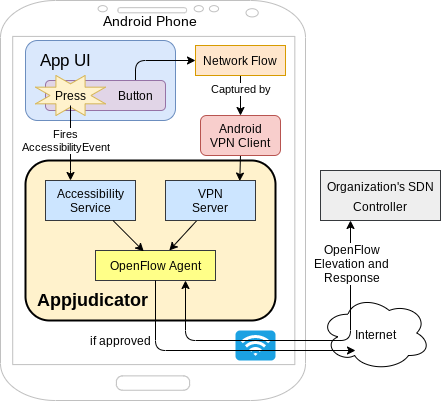
\includegraphics[width=.6\textwidth]{component-diagram.png}
    \caption{Diagram of component interactions.}
    \label{fig:component-diagram}
\end{wrapfigure}

The networking component of \textsc{Appjudicator} utilizes Android's built-in
API for redirecting network traffic, the VPN
Service~\cite{googledevelopers2020vpn}. We direct Android's built-in
VPN client to connect to a custom VPN server running on the Android device
itself. With the user's permission we can route all traffic through this VPN,
allowing us to capture all network flows entering and exiting the device. We implement a
low-level system for intercepting packets, inspecting their contents, and making
decisions on whether to forward the packets to their intended destination or
drop them.

Once activated, the VPN service runs in the background and receives packets from
the operating system through a file interface. An application can read from this
interface to get packets from the networking stack as raw byte arrays in the
same way it would read from any other file. Likewise we can write to the
interface like a file to send raw data to the network. \textsc{Appjudicator}
manages connections and forwards allowed packets to their remote destination
using Java sockets.

The VPN service provides network context that can be used by the SDN agent. For
example, the destination IP address, protocol, payload size, initiating
application, and full packet payload can all be used to enforce fine-grained SDN
rules.
% TODO write about how we get the initiating application in Implementation

Apps are likely to make some kinds of network requests independent of user
interaction, for example automatically fetching weather data from the Internet
every hour. To account for this we profile known-benign apps using tcpdump to
see what sort of requests they make independently over several hours with no
interaction, and record these flows in a default-allow list. Then, during normal
operation of the app if we receive a network flow that is not on this list
\textit{and} was not initiated by a user interaction we can investigate it
further.

\subsection{Accessibility Service}
\label{sec:approach-accessibility-service}

The user interface monitoring component is implemented as an Accessibility
Service, using Android's API for simulating and responding to user interaction
with the UI~\cite{googledevelopers2020}. This service runs in the background and
receives information from accessibility events asynchronously. These
accessibility events contain data about what action was performed (clicking,
swiping, entering text, \textit{etc}.) and what UI element was the target of the
action. This UI data is the key to the central idea of \textsc{Appjudicator}: it
lets us associate a network flow with the UI interaction that initiated it.

% Move this paragraph to background
Android accessibility services break the operating system's normally strong
sandboxing principles by their ability to read and interact with anything
displayed on the screen~\cite{kalysch2018}. For security reasons, Android
requires any accessibility service to be enabled manually by the user in the
settings app. But once the service is enabled it can run continuously in the
background, receiving accessibility events from almost any UI interaction in any
app.

\subsection{Software-defined Networking}
\label{sec:sdn-rule-cache}

We combine networking control from the VPN service with UI monitoring from the
accessibility service to create a context-enhanced SDN agent.
Figure~\ref{fig:component-diagram} shows how each of \textsc{Appjudicator}'s
components integrate with the other aspects of the phone environment. The app
acts as an OpenFlow-compatible agent while receiving UI interaction data from
the accessibility service and network flows from the VPN service. It enforces
policy on the device, forwarding, dropping, or elevating packets based on rules
received from the organization's OpenFlow controller server.

To do this, we implement a subset of the OpenFlow protocol, including logic for
caching rules from the controller server, inspecting packets, and enforcing
rules. The OpenFlow agent performs all the standard behavior of an SDN agent:
caching rules, forwarding packets according to rules, and elevating flows to the
controller server.

A flow's initiating UI interaction is determined by temporal association. When a
new flow is intercepted \textsc{Appjudicator} looks up the most recent UI
interactions from the same application to see if there was a likely initiator,
such as a button press, within the last two seconds. We send as much data about
any potential matches as we can fit into a packet-in OpenFlow message (see
Section~\ref{sec:openflow-protocol}) to the SDN controller when a flow is
elevated, to provide additional context.

\newpage
